% Chapter Template

\chapter{系统结构设计} % Main chapter title

\label{Chapter2} % Change X to a consecutive number; for referencing this chapter elsewhere, use \ref{ChapterX}

%----------------------------------------------------------------------------------------
%	SECTION 1
%----------------------------------------------------------------------------------------


数据库的基本架构与实验要求基本相同。我们将主要的模块分为了记录管理模块(RM\_Manager),系统管理模块(SM\_Manager),查询解析模块(QL\_Manager),语句解析模块(Parse\_Manager)和索引模块(IX\_Manager)。

\begin{figure}[H]
\centering
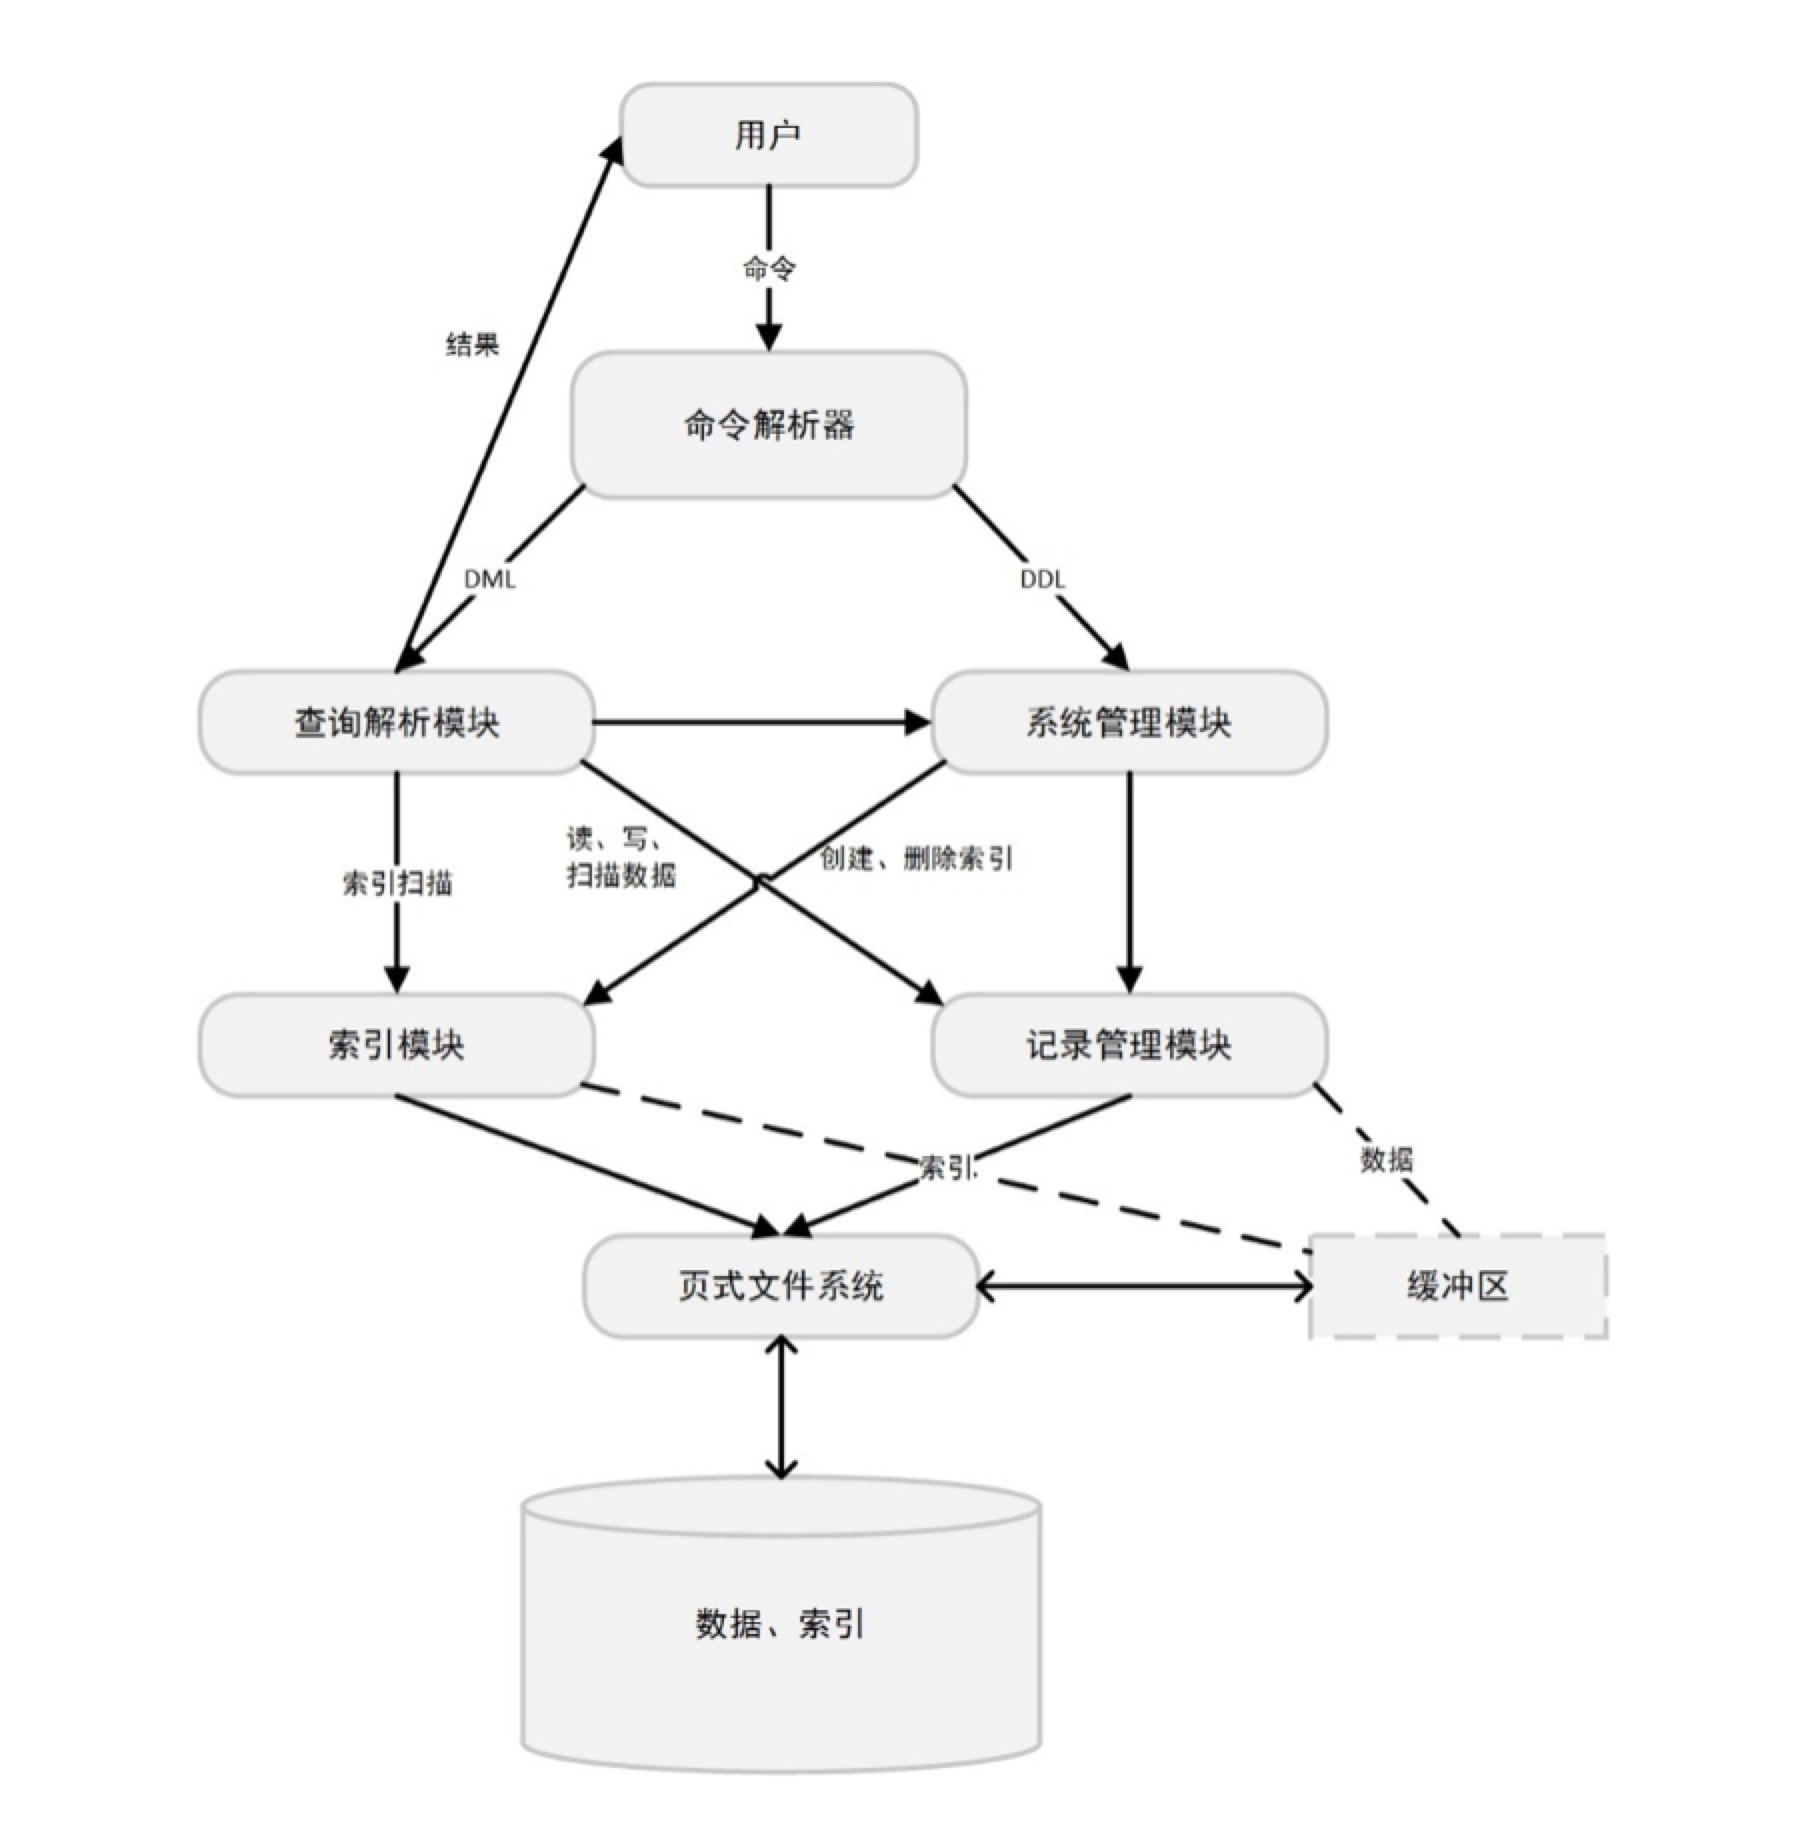
\includegraphics[width=5in]{Figures/structure.jpg}
\end{figure}

每个数据库在存储空间上对应于一个文件夹,其中包含很多文件,对应于每一个表。每个数据库中有两个专用的表,分别为attrcat与tablelist。 attrcat表用于存储当前数据库中每个用户表的属性值,而tabellist表用于存储当前数据库所有用户表的信息。

数据库中每个表中的记录大小可以不一样,在新建表时指定,但是同一个表中的记录记录是定长的。在每个表中,第一页为存储文件信息的页,后续的各页用于存储记录。为了方便索引,在每页中页头部分记录当前页的使用情况。

下图可以表示出我们设计的数据库的基本结构:

\begin{figure}[H]
\centering
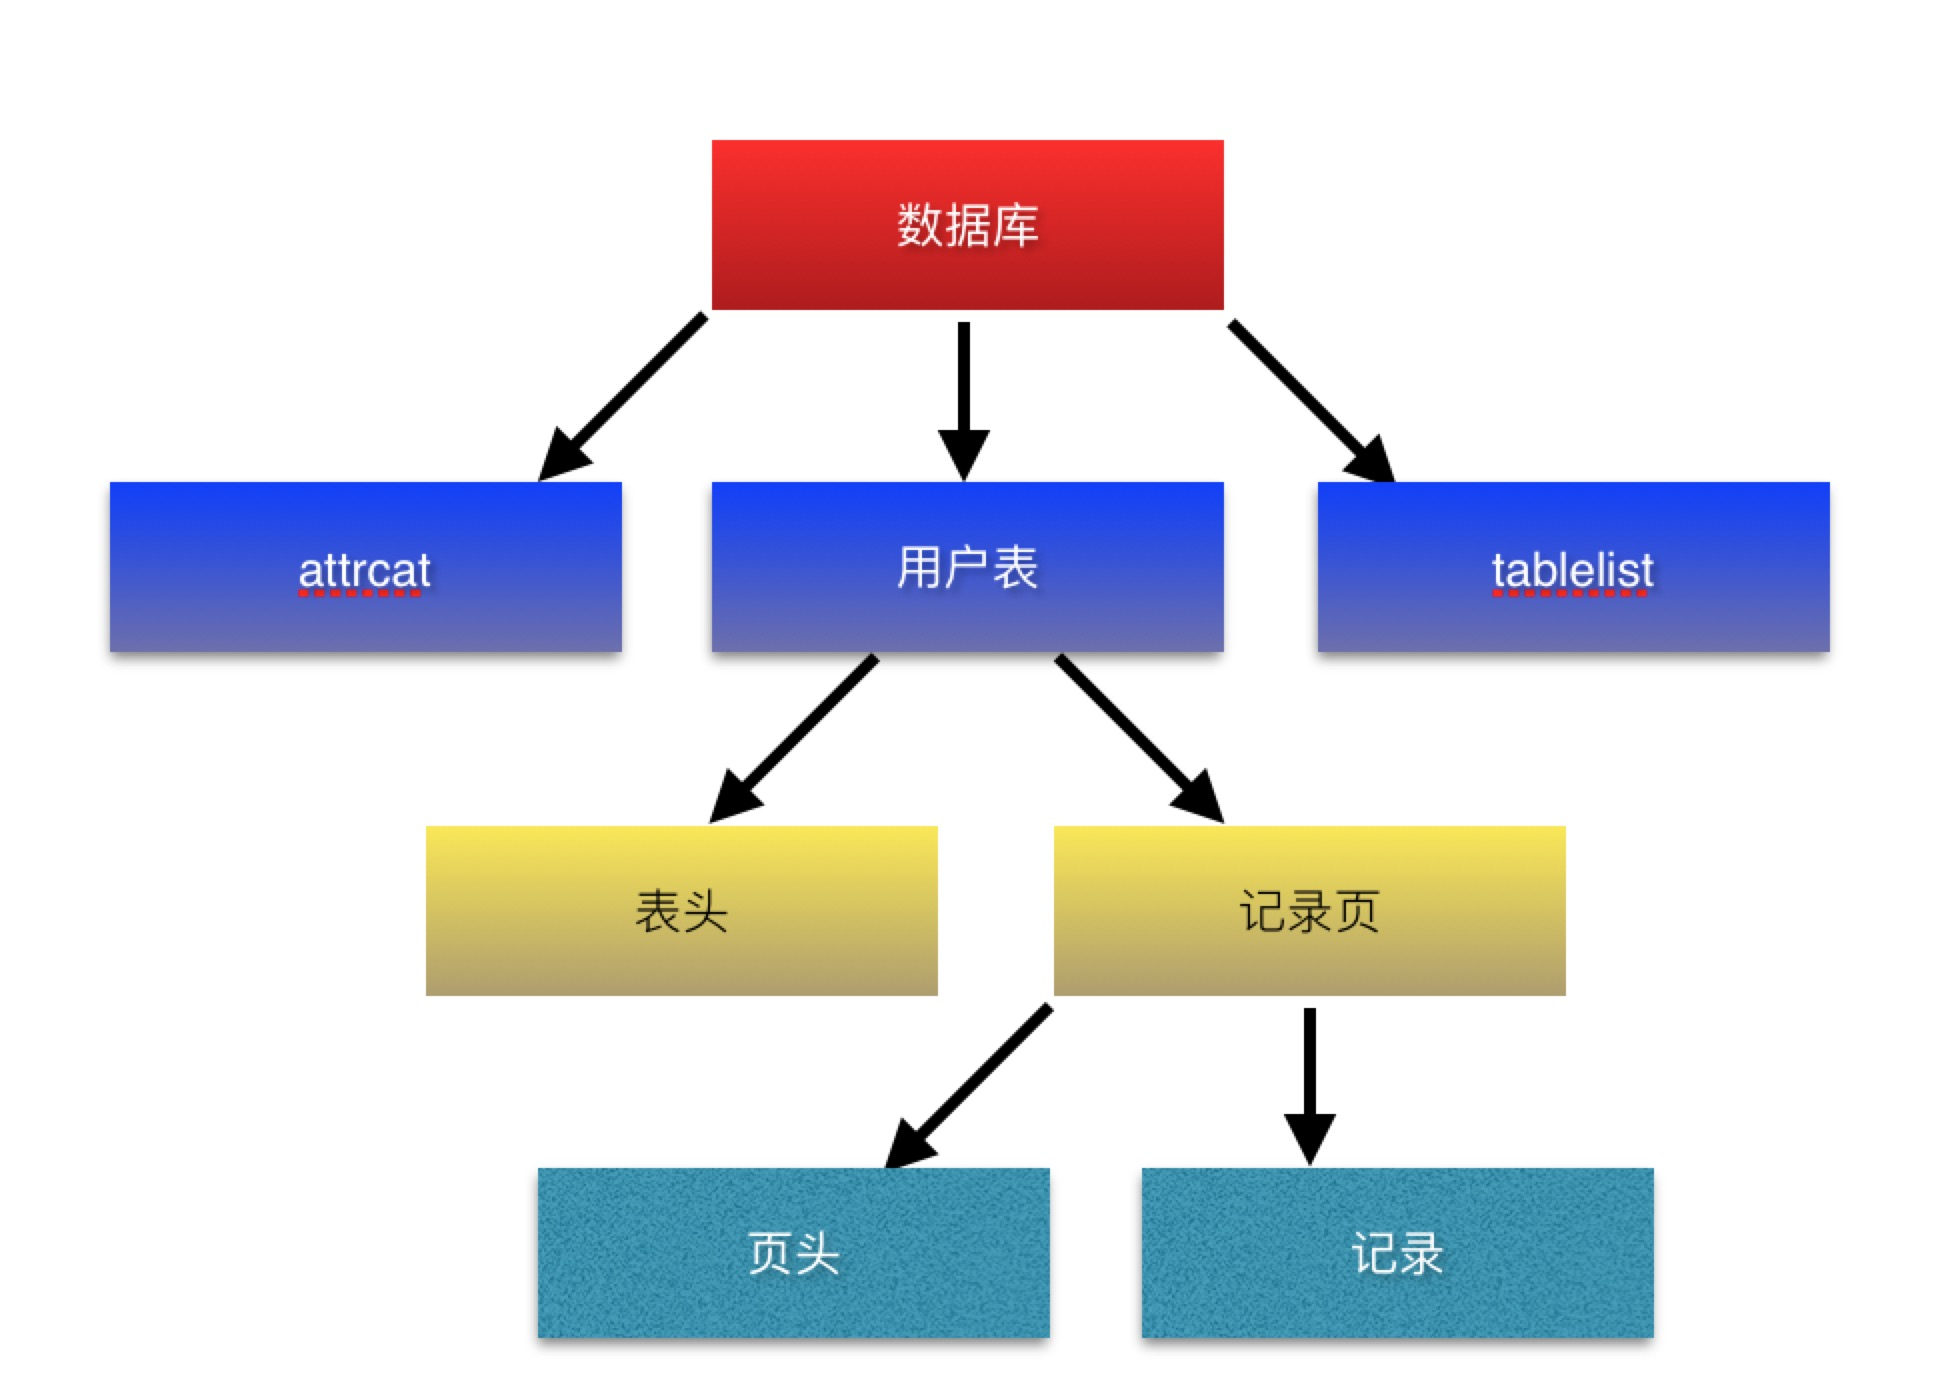
\includegraphics[width=5in]{Figures/DB.jpg}
\end{figure}

